%!TEX encoding = UTF-8 Unicode
%!TEX TS-program = xelatex
%!BIB TS-program = biber

% paper for BeLLS
\documentclass[11pt,twoside]{article}
%!TEX encoding = UTF-8 Unicode
% packages and settings for BeLLS
% all packages are available in standard LaTeX distributions such as MacTeX 2016

% page layout (text area is 126mm, 196mm)
\usepackage[papersize={17cm,24cm},margin=22mm,top=17mm,headsep=5mm]{geometry} 

\usepackage{xltxtra} % extras for XeLaTeX
\usepackage{verbatim} % verbatim input
\usepackage{titling} % customize title
\usepackage{csquotes} % context sensitive quotes
\usepackage{upquote} % allow correct quotes in verbatim
\usepackage[bottom]{footmisc} % put footnotes down at the bottom margin
\usepackage[svgnames]{xcolor} % color pictures with SVG names
\usepackage{graphicx} % \includegraphics
\usepackage{enumitem} % customize lists
%\setitemize{noitemsep,topsep=0pt,parsep=0pt,partopsep=0pt}
\setitemize{itemsep=2pt,topsep=4pt,parsep=0pt,partopsep=0pt}
\usepackage{covington}  % for numbered linguistic examples

%\usepackage[english]{babel} % multilinguality
\usepackage{polyglossia} % newer alternative to babel
\setdefaultlanguage{english} % see http://ctan.uib.no/macros/xetex/latex/polyglossia/polyglossia.pdf

\setmainfont[Mapping=tex-text,Ligatures=TeX,Scale=1.0]{Linux Libertine O} 
\setmonofont[Mapping=tex-text,Scale=MatchLowercase,LetterSpace=-2.0]{DejaVu Sans Mono}
\renewcommand{\baselinestretch}{1.04} % stretch distance between baselines
\frenchspacing % reduce space after sentence-final punctuation
\date{}
\setlength{\parindent}{1em}
\clubpenalty = 10000
\widowpenalty = 10000
\hfuzz = 2pt  % No warnings about margin overhangs less than this amount.
%\setlength{\belowcaptionskip}{-1.2em}

\usepackage[backend=biber, style=authoryear, citestyle=authoryear-comp, maxcitenames=2, maxbibnames=50, language=auto, isbn=false, url=false]{biblatex} % new alternative to bibtex
\setlength{\bibhang}{\parindent}
\usepackage[breaklinks,colorlinks,urlcolor=black,citecolor=black,linkcolor=black]{hyperref} % pagebackref incompatible with biblatex

\usepackage[compact,noindentafter]{titlesec} % customize section headings
\titlespacing{\section}{0pt}{2.7mm}{1.5mm} % left indent, space before, space after
\titlespacing{\subsection}{0pt}{2mm}{1pt}
\titlespacing{\subsubsection}{0pt}{1.2mm}{0.5pt}

\newcommand\Volume{N} % BeLLS Volume number
\newcommand\Voleditors{ajgupta@ucsd.edu, jsc078@ucsd.edu}
\newcommand\Voltitle{The book title}
\newcommand\VolISBN{N}
\newcommand\VolDOI{N}

%\usepackage{natbib}
%\usepackage{fullname}
%\bibliographystyle{fullname} % chicago or spbasic or spmpsci or spphys
%\setlength{\bibhang}{-0.5em}
%\setlength{\bibsep}{0mm}
%\let\bibfont=\small

% footnote without number
\newcommand\blfootnote[1]{
  \begingroup
  \renewcommand\thefootnote{}\footnote{\hspace{-2.4em} #1}%
  \addtocounter{footnote}{-1}
  \endgroup
}

% customize title
\renewcommand{\maketitle}
  {\bgroup\setlength{\parindent}{0pt}
   \begin{flushleft}
    \textbf{\LARGE{\ \\ \vspace{20mm}\strut\thetitle\strut}\vspace{2mm}}
    
    {\Large\theauthor}
  \end{flushleft}\egroup\vspace{18mm}
}

% customize abstract
\renewenvironment{abstract}
  {\noindent\small %\quotation
  {\noindent{\large\textbf\abstractname. }%\par\nobreak\smallskip
  \thispagestyle{plain}
  %\blfootnote{In: \emph{Volume title,} edited by Jan Editor and Ed Janitor. BeLLS Vol. N (2017), DOI N. Open Access under the terms of CC-BY-NC-4.0.}
  }}
  {}
    
% command in which to embed tabular material in numbered example
% use: \begin{example}\extab\begin{tabular ...
\newcommand{\extab}[2][-0.69\baselineskip]{ 
   \parbox[t]{.9\textwidth}{
     \setlength{\tabcolsep}{1.3pt} % use small space between columns
     \vspace{#1}
     #2
    }
}

% command to put ref in parentheses
\newcommand{\refp}[1]{(\ref{#1})}

% customize page headers
\usepackage{fancyhdr}
\pagestyle{fancy}
\renewcommand{\headrulewidth}{0.4pt}
\fancyhead{}  \fancyfoot{} %clear
\makeatletter % necessary for commands with @
  \fancyhead[RO]{\small\textit{\@title}}
  \fancyhead[LE]{\small\textit{\@author}}
\makeatother
%\fancyhead[RE]{\small BeLLS Vol. \Volume}
 % no footer
\setlength{\headheight}{20.68pt} % room for two lines
\fancypagestyle{plain}{% first page of chapter
 %\fancyhead[L]{}
 \fancyhead[L]{\footnotesize  \emph{CSE253 HW1} ajgupta@ucsd.edu, jsc078@ucsd.edu} % comment to keep the normal header
  \fancyhead[C,R]{}
  %\renewcommand{\headrulewidth}{0pt} % comment to keep rule
  \fancyfoot{} % comment to put page number at bottom
  }

 % load packages, set parameters, define commands

% use the following packages if needed (if not, you can omit loading these)
\usepackage{synttree} % for drawing syntactic trees
\branchheight{2.5em} \childsidesep{0.5em} % synttree settings
\usepackage{avm} % for drawing attribute-value matrices

\usepackage{amsmath}
\usepackage{graphicx}
\usepackage{hyperref}
\usepackage{listings}
\usepackage{subcaption}
\usepackage{enumitem}
\usepackage{amssymb}
\usepackage{float}
\usepackage{physics}
\usepackage[toc,page]{appendix}

\usepackage{color}

\definecolor{codegreen}{rgb}{0,0.6,0}
\definecolor{codegray}{rgb}{0.5,0.5,0.5}
\definecolor{codepurple}{rgb}{0.58,0,0.82}
\definecolor{backcolour}{rgb}{0.95,0.95,0.92}
 
\lstdefinestyle{mystyle}{
    backgroundcolor=\color{backcolour},   
    commentstyle=\color{codegreen},
    keywordstyle=\color{magenta},
    numberstyle=\tiny\color{codegray},
    stringstyle=\color{codepurple},
    basicstyle=\footnotesize,
    breakatwhitespace=false,         
    breaklines=true,                 
    captionpos=b,                    
    keepspaces=true,                 
    numbers=left,                    
    numbersep=5pt,                  
    showspaces=false,                
    showstringspaces=false,
    showtabs=false,                  
    tabsize=4
}
 
\lstset{style=mystyle}


%\usepackage{epstopdf} % for eps graphics

\author{Ajitesh Gupta, Jean Choi} % no affiliation
\title{Studying regression and regularization using binary and multiclass classification on MNIST dataset.} % do not capitalize every open class word
%\addbibresource{sample.bib} % the bib file

\hyphenation{lem-mat-iz-at-ion uni-code ADVdeg Hel-ge}
\graphicspath{{pics/}} % the pictures folder

\begin{document}
\maketitle

\begin{abstract}
In this assignment we looked at two regression techniques namely Logistic regression and Softmax regression. We then applied these to solve the problem of binary classification and multiclass classification respectively on the MNIST handwritten dataset. We also studied the effect of regularization by implementing L1 and L2 regularization on both of them and compared between them.\\

For logistic regression without regularization, we achieved \textcolor{red}{\textbf{96.7 \%}} accuracy for 2 $vs$ 3 and \textcolor{red}{\textbf{87.3 \%}} for 2 $vs$ 8, in classifying the number 2. There were 4005 training samples, of which 405 were the hold-out set and the accuracy is with respect to 426 training samples in 2 $vs$ 3 case. There were 3851 training samples, of which 351 were the hold-out set and the accuracy is with respect to 426 training samples in 2 $vs$ 8 case.\\

Using regularization, we achieved \textcolor{red}{\textbf{97.8 \%}} accuracy for 2 $vs$ 3 in both L1 and L2 regularization using $\lambda$ values of 1 and 10 respectively.\\

In Softmax regression we achieved \textcolor{red}{\textbf{86.7 \%}} accuracy using L1 regularization with a $\lambda$ value of 1. There were 20,000 training samples out of which 2000 were used as a hold-out(validation) set. The test set was also comprised of 2000 samples.

\end{abstract}

\section{Introduction}


\subsection{Logistic Regression}

Logistic regression uses sigmoid function, which ensures that the prediction falls within the range of 0 and 1. Thus, it can be used for classifying objects into two classes and in this homework, it will be used to classify the numbers either as 2 or not.\\

To use logistic regression, I first need to derive the gradient. The derived gradient can used for calculating the prediction, shifting the weights, and also measuring the loss.\\

The following equation is given:\\
\begin{equation}
E^{n} = -t^{n}\log y^{n} - (1 - t^{n})\log (1 - y^n)
\end{equation}
whereas,
\begin{equation}
y^{n} = g_{w}(x^{n}) = \frac{1}{1 + e^{-w^{T}x^{n}}}
\end{equation}

Thus equation (1) can be rewritten as:\\
\begin{equation}
\begin{split}
E^{n} & = -t^{n}\log y^{n} - (1 - t^{n})\log (1 - y^n)\\
& = (t^{n} - 1)\log e^{-w^{T}x^{n}} + \log (1 + e^{-w^{T}x^{n}})\\
& = (1 - t^{n})(w^{T}x^{n}) + \log (1 + e^{-w^{T} x^{n}})\\
\end{split}
\end{equation}

Differentiate $E^{n}$ with respect to $w_{j}$:\\
\begin{equation}
\begin{split}
\pdv{E^{n}}{w_{j}} & = (1 - t^{n})\pdv{}{w_{j}} (w_{j} x^{n}_{j}) + \pdv{}{w_{j}}\log (1 + e^{-w_{j} x^{n}_{j}})\\
& = (1 - t^{n})x^{n}_{j} + \frac{1}{1 + e^{-w_{j} x^{n}_{j}}} (-x^{n}_{j})e^{-w_{j} x^{n}_{j}}\\
& = -x^{n}_{j}(t_{n} - \frac{1}{1 + e^{-w_{j} x^{n}_{j}}})\\
& = -x^{n}_{j}(t_{n} - y_{n})\\
\end{split}
\end{equation}

\begin{equation}
\therefore -\pdv{E^{n}}{w_{j}} = (t_{n} - y_{n})x^{n}_{j}
\end{equation} 

\subsection{Regularization}


\subsection{Softmax Regression}
In softmax regression we solve a multi-class classification problem as opposed to the logistic regression where we have binary classification. The classification function involves an exponential normalized by a sum of exponentials (each calculated using weight vectors of different classes).
\begin{equation}
\begin{split}
J(w) &= -\sum^m_{i=1}\sum^K_{k=1}\{ t^{(i)} = k \}\log p(y^{(i)} =  k \mid x^{(i)} ;w)\\
& = - \sum^m_{i=1} \sum^K_{k=1} \{t^{(i)}=k\} \log \frac{e^{w^T_k x^{(i)}}}{\sum^K_{l=1}e^{w^T_l x^{(i)}}} \\
\end{split}
\end{equation}

Using the logarithm rule $ln(\frac{a}{b}) = ln(a)-ln(b)$ :
\begin{equation}
\begin{split}
J(w)  =- \sum^m_{i=1} \sum^K_{k=1} \{t^{(i)}=k\}[\log e^{w^T_kx^{(i)}}-\log \sum^K_{l=1}e^{w^T_lx^{(i)}}]\\
\end{split}
\end{equation}

The partial derivative of J with respect to $w_{k}$ is:
\begin{equation}
\bigtriangledown_{ w_k }J( w ) = - \sum^m_{i=1} \{t^{(i)}=k\}[x^{(i)}-\frac{1}{\sum^K_{l=1}e^{w^T_lx^{(i)}}}e^{w^T_kx^{(i)}}x^{(i)}]
\end{equation}

Now we see that for the $K^{th}$ category only one element in $\bigtriangledown_{ w_k} \sum^K_{l=1}e^{w^T_kx^{(i)}}$ is nonzero, that is $e^{w^T_kx^{(i)}}$. Hence we can replace p back to get:

\begin{equation}
\bigtriangledown_{ w_k }J( w ) = -\sum^{m}_{i=1} [x^{(i)} (\{ t^{(i)} = k \} - p(y^{(i)} =  k \mid x^{(i)} ; w) ) ]
\end{equation}

As such for a particular value of i = j

\begin{equation}
\bigtriangledown_{ w_{jk} }J( w ) = - [x_{j} ( t_{k} - y_{k})] 
\end{equation}

\section{Methods}

\subsection{Logistic Regression}

To achieve the classification of high accuracy with computation efficiency, the given batch gradient descent algorithm and early stopping were implemented.\\ 

When images are read in, they are stored as arrays of values ranging from 0 to 255. These will be referred as image vectors from now on. To prevent overflow or computations using very large numbers, the image vectors were divided by 255, element-wise.\\

The parameters used in gradient descent such as number of epochs, $m$, initial learning rate, $nu$, and metaparameter, $T$, were given values based on experiments.\\

\begin{itemize}
\item Gradient:\\
The gradient derived from \textbf{1.1} was used. The weight vector was set to the same dimensions as an image vector.\\

\item Gradient descent:\\
The weight vector, which was initially set to all zeros, was updated at each iteration using gradient descent:\\
\begin{equation}
w_{t+1} = w_{t} - \eta \sum_{n = 1}^{N} \nabla E^{n}(w)
\end{equation}

\item Loss:\\
Loss function is a way to measure how the current weight vector is effective in classifying the numbers. The weight vector can be updated with respect to the loss. Following is the average of the loss:\\
\begin{equation}
E(w) = -\sum_{n = 1}^{N} t^{n}\log y^{n} - (1 - t^{n})\log (1 - y^n)
\end{equation}

\item Percent correct classification:\\
Percent correct classification is another way to see how well the weight vector is doing:\\
\begin{equation}
p = \frac{\lbrace t^{n} = 1, y^{n} \geq 0.5\rbrace + \lbrace t^{n} = 0, y^{n} < 0.5 \rbrace}{N}
\end{equation}

\item Early stopping:\\
Early stopping was implemented based on the loss on hold-out set. At each iteration, $m$, the loss is calculated on the hold-out set with respect to the current weight vector obtained from the rest of the training set. If there are originally $N + \alpha$ training samples, then the weight vector is obtained from performing gradient descent on $N$ samples. The the loss is calculated on $\alpha$ samples. In this homework, $\alpha$ was chosen to be \textit{roughly} 10\% of the entire training set, because $\alpha$ needs to be an integer. For 2 $vs$ 3, there were a total of 4005 training samples, of which 405 were chosen to be the hold-out set. For 2 $vs$ 8, there were a total of 3851 training samples, of which 351 were chosen to be the hold-out set.\\

The iteration stops when the loss has not been decreasing for more than 3 steps. In the first few steps, the loss is pretty high due to the small number of iterations which results in less distinguishable weight vector. Thus the early stopping is applied only after first 5 steps.\\

\item Minibatch:\\
The weight vector was updated every mini-iteration i.e. whenever the number of training samples processed so far is a multiple of $1/10 ^{th}$ of the total number. This was implemented using simple \textbf{if} statement in the gradient descent algorithm.\\

\end{itemize}



\subsection{Regularization}
The two regularization methods used were L1 and L2. L1 regularization penalizes on the sum of the weight vector values itself whereas the L2 regularization penalizes on the squared sum of the weight vector values.

\begin{itemize}

\item{L1 Regularization}\\
The cost function used was  as follows:

\begin{equation}
E(w) = -\sum_{n = 1}^{N} t^{n}\log y^{n} - (1 - t^{n})\log (1 - y^n) + \lambda\sum_{i = 1}^{D}w_{i}
\end{equation}

Differentiating this w.r.t. $w_{i}$ and using previously derived update rule, we get the update rule as:
\begin{equation}
w_{t+1} = w_{t} - \eta \sum_{n = 1}^{N} \nabla E^{n}(w) + \lambda
\end{equation}

\item{L2 Regularization}\\
The cost function used was as follows:

\begin{equation}
E(w) = -\sum_{n = 1}^{N} t^{n}\log y^{n} - (1 - t^{n})\log (1 - y^n) + \lambda w^{T}w
\end{equation}
Differentiating this w.r.t. $w_{i}$ and using previously derived update rule, we get the update rule as:
\begin{equation}
w_{t+1} = w_{t} - \eta \sum_{n = 1}^{N} \nabla E^{n}(w) +\lambda\sum_{i = 1}^{D}w_{i}
\end{equation}
\end{itemize}

\subsection{Softmax Regression}
\begin{itemize}
\item Gradient:\\
The gradient derived from \textbf{1.3} was used. The weight vector was set to the same dimensions as an image vector.\\

\item Gradient descent:\\
The weight vector, which was initially set to all zeros, was updated at each iteration using gradient descent:\\
\begin{equation}
w_{t+1} = w_{t} - \eta \sum_{n = 1}^{N} \nabla E^{n}(w)
\end{equation}

\item Loss:\\
Loss function is a way to measure how the current weight vector is effective in classifying the numbers. The weight vector can be updated with respect to the loss. Following is the average of the loss:\\
\begin{equation}
E = -\frac{1}{n}\sum_{n}^{} \sum_{k=1}^{c}{t_{k}}^{n}\log{y_{k}}^{n}
\end{equation}

\item Percent correct classification:\\
Percent correct classification is another way to see how well the weight vector is doing:\\
\begin{equation}
p = \frac{\sum_{n=1}^{N}\lbrace t^{n} = k, y^{n} \simeq k\rbrace}{N}
\end{equation}
\end{itemize}





\section{Results and Discussions}

\subsection{Logistic Regression}

For all the following calculations and plots, $m = 500$, $\eta = 0.01$, $T = 2$, and $target = 2$ were used.\\
Green represents the training set, blue the hold-out set, and red the test set.\\

\begin{enumerate}[label=(\alph*)]

\item \textbf{Loss Function}\\
The average loss function was used for calculating the loss.

\begin{itemize}
  \item Without early stopping
  
  \begin{figure}[H]
  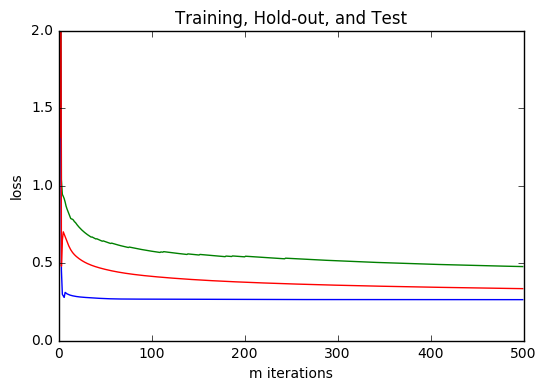
\includegraphics[width=0.6\textwidth]{nonstop_all_loss}
  \centering
  \caption{}
  \label{fig:4_2}
  \end{figure}
  
  In general, the loss decreased for all three sets, whereas the loss for the training set is higher than the other two. As the number of iterations, $m$, is increased, the training and test loss keep decreasing while the hold-out loss becomes nearly constant.\\
  
  The loss of hold-out set tends to be similar to that of test set rather than that of training set.\\
  
  \item With early stopping
 
  \begin{figure}[H]
  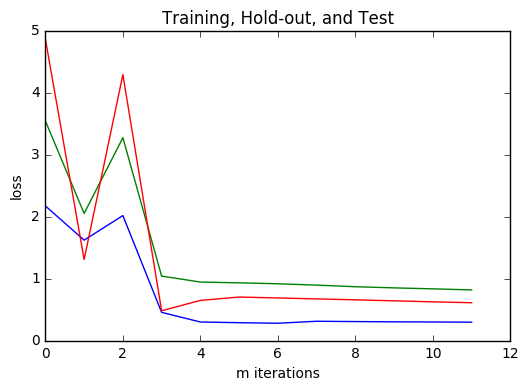
\includegraphics[width=0.6\textwidth]{stop_all_loss}
  \centering
  \caption{}
  \label{fig:4_2}
  \end{figure}
  
  With early stopping implemented, it stops at $11^{th}$ iteration. The iteration stops when it has not been decreasing for more than 3 steps. In the first few steps, the loss is pretty high due to the small number of iterations which result in less distinguishable weight vector. Thus the early stopping is applied only after first 5 steps.\\
  
  \item With minibatch and early stopping
  
  \begin{figure}[H]
  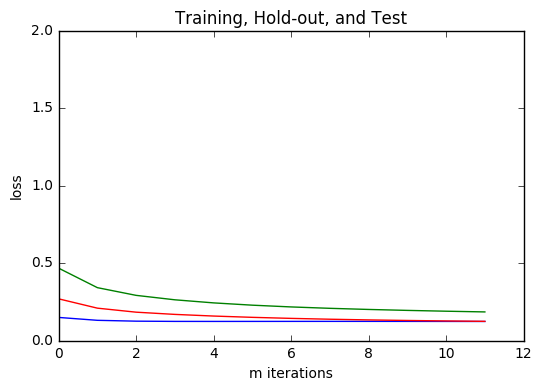
\includegraphics[width=0.6\textwidth]{stop_mini_all_loss}
  \centering
  \caption{}
  \label{fig:4_2}
  \end{figure}
  
  With minibatch and early stopping implemented, it stops at $11^{th}$ iteration. When the minibatch is applied, the loss are generally smaller than those using routine batch. Also the graphs look smoother, i.e. not a lot of spikes, as apparent in the comparison to the previous figure.\\
  
  Also, the loss of hold-out set is now even more similar to that of test set. Thus it can be said that hold-out set does work as a good stand-in for the test set for this case.\\
  
\end{itemize}

\item \textbf{Percent Correct Classification}\\

The "error rate" was calculated using $100 - accuracy$, whereas the $accuracy$ was calculated with the given description.\\
  \begin{figure}[H]
  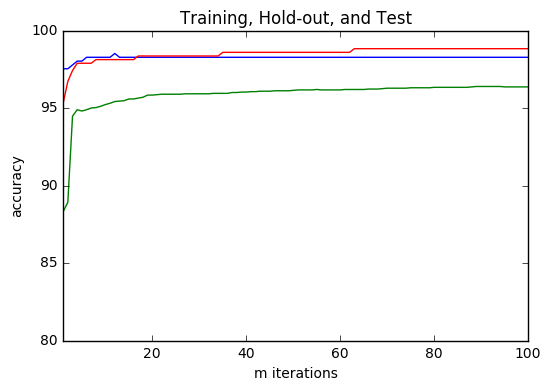
\includegraphics[width=0.6\textwidth]{acc_all}
  \centering
  \caption{}
  \label{fig:4_2}
  \end{figure}
  
  The error rate for the training and test sets keep decreasing while the error rate for hold-out set takes a dip and then goes almost constant.\\

%----------------------------------------
\item \textbf{2 vs 8}

\begin{itemize}
  \item Without early stopping
  
  \begin{figure}[H]
  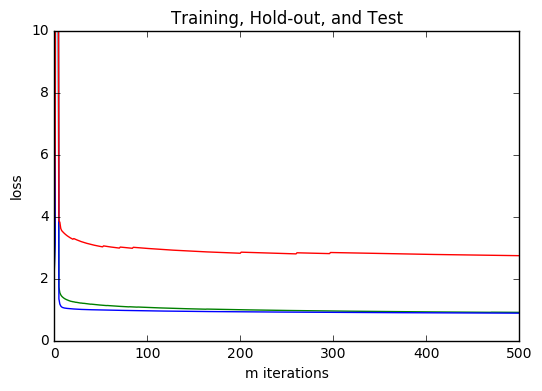
\includegraphics[width=0.6\textwidth]{cnonstop_all_loss}
  \centering
  \caption{}
  \label{fig:4_2}
  \end{figure}
  
  In general, the loss decreased for all three sets, whereas the loss for the test set is higher than the other two. As the number of iterations, $m$, is increased, the training and test loss keep decreasing while the hold-out loss becomes nearly constant.\\
  
  The loss of hold-out set tends to be similar to that of training set rather than that of test set.\\
  
  \item With early stopping
 
  \begin{figure}[H]
  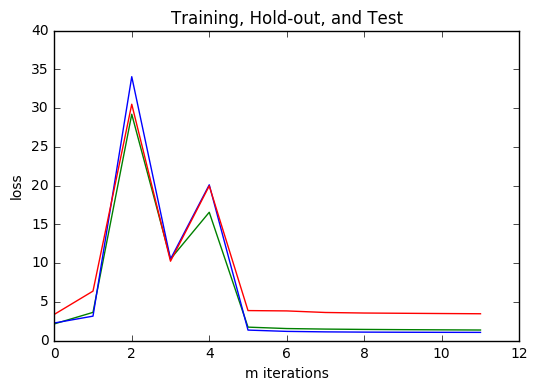
\includegraphics[width=0.6\textwidth]{cstop_all_loss}
  \centering
  \caption{}
  \label{fig:4_2}
  \end{figure}
  
  With early stopping implemented, it stops at $11^{th}$ iteration. The iteration stops when it has not been decreasing for more than 3 steps. In the first few steps, the loss is pretty high due to the small number of iterations which result in less distinguishable weight vector. Thus the early stopping is applied only after first 5 steps.\\
  
  \item With minibatch and early stopping
  
  \begin{figure}[H]
  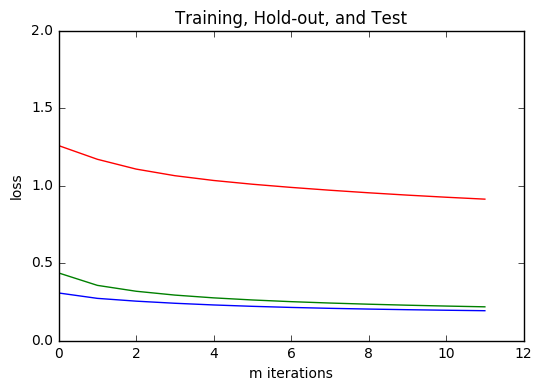
\includegraphics[width=0.6\textwidth]{cstop_mini_all_loss}
  \centering
  \caption{}
  \label{fig:4_2}
  \end{figure}
  
  With minibatch and early stopping implemented, it stops at $11^{th}$ iteration. When the minibatch is applied, the loss are generally smaller than those using routine batch. Also the graphs look smoother, i.e. not a lot of spikes, as apparent in the comparison to the previous figure.\\
  
  Also, the loss of hold-out set is still more similar to that of training set. Thus it can be said that hold-out set does NOT work as a good stand-in for the test set for this case.\\

  \item Percent correct classification
  
  \begin{figure}[H]
  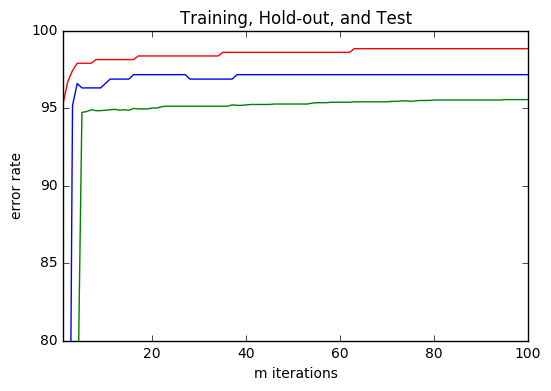
\includegraphics[width=0.6\textwidth]{cacc_all}
  \centering
  \caption{}
  \label{fig:4_2}
  \end{figure}

\end{itemize}

\item \textbf{Weight Vectors}

\begin{itemize}

  \item Weight Vectors
  \begin{figure}[H]
  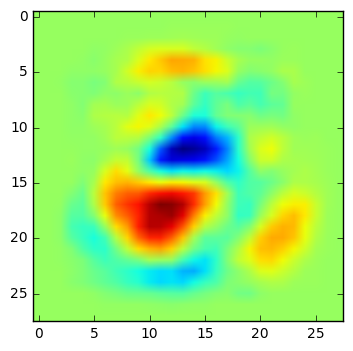
\includegraphics[width=0.45\textwidth]{2vs3_weight}
  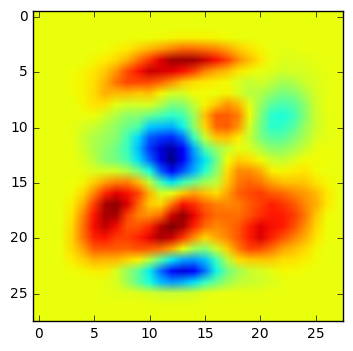
\includegraphics[width=0.45\textwidth]{2vs8_weight}
  \centering
  \caption{Left: 2 vs 3 Right: 2 vs 8}
  \label{fig:4_2}
  \end{figure}
  
  \item Difference Weight Vector
  \begin{figure}[H]
  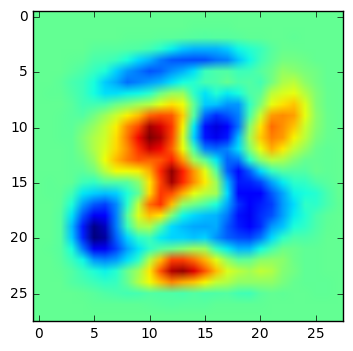
\includegraphics[width=0.45\textwidth]{diff_weight}
  \centering
  \caption{Difference}
  \label{fig:4_2}
  \end{figure}
  
  Where the values are high, the numbers are distinctive. On the other hand, if the values are low, they are similar. Thus the red colors in the difference image represent the part where 2, 3, and 8 are all distinctive. The blue colors represent the part where 3 and 8 are similar but different from 2. Since 2, 3, and 8 are a particular set of numbers that can easily be mistaken for one another, this difference image/weight vector can be used to distinguish them.
  
\end{itemize}

\end{enumerate}

\subsection{Regularization}
\begin{enumerate}[label=(\alph*)]

\item \textbf{Percent correct vs. Lambda}\\
In case of L2 regularization we see that the lambda values do not have so much of an effect on the accuracy. But in case of L1 regularization we see that accuracy is higher for lower value of lambda.
\begin{figure}[H]
  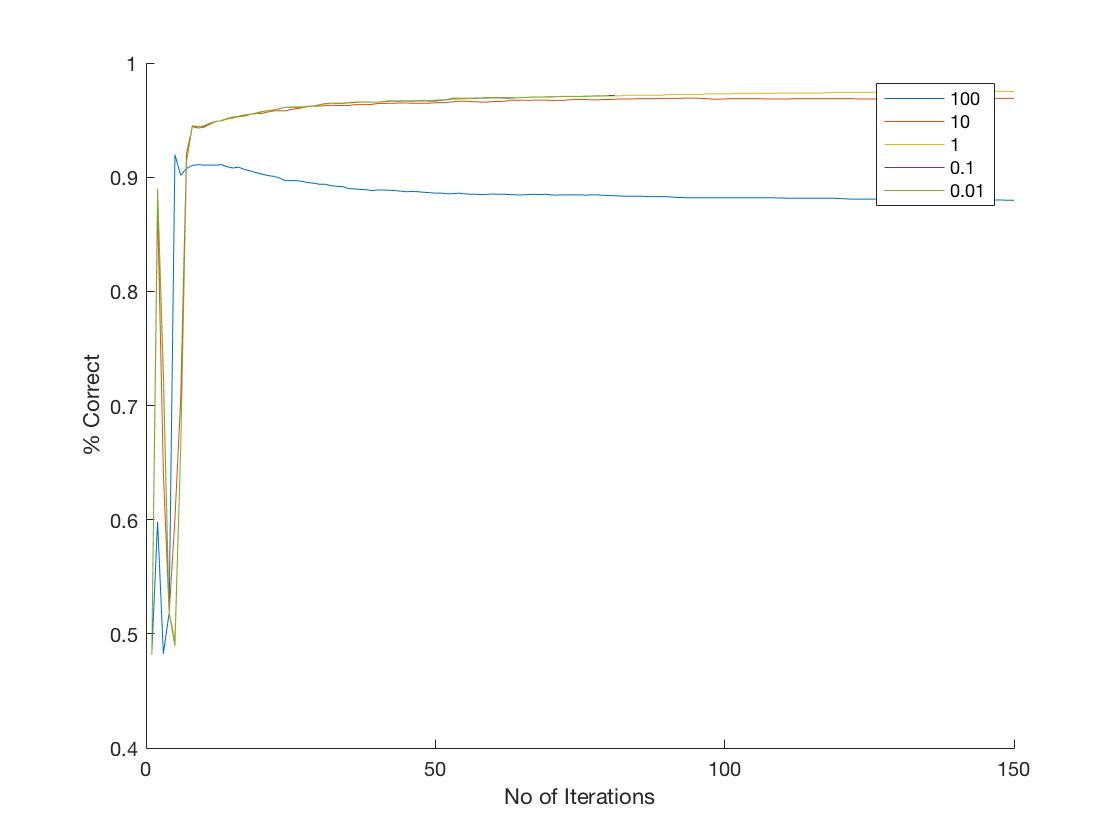
\includegraphics[width=0.45\columnwidth]{5b_l1}
  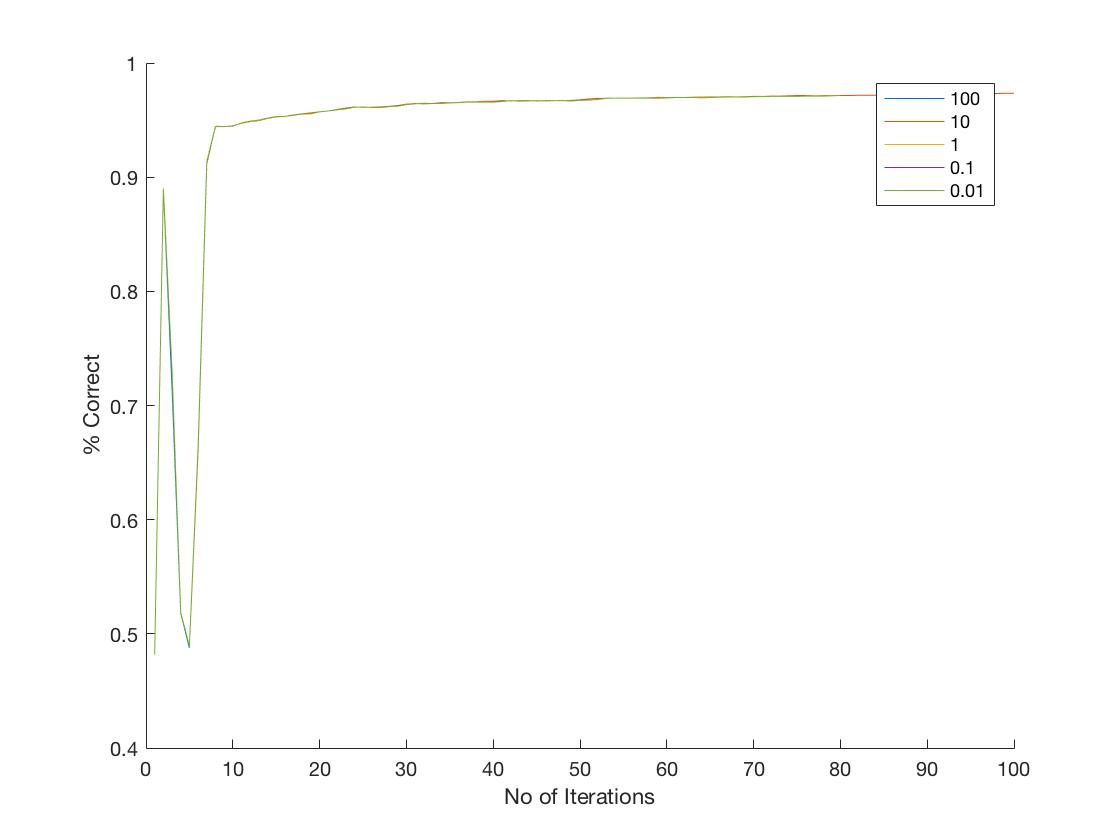
\includegraphics[width=0.45\columnwidth]{5b_l2}
  \centering
  \caption{Left: L1 Right: L2}
  \label{fig:5_b}
  \end{figure}
  
\item \textbf{Weight Vector Magnitude vs. Lambda}\\
We see that as expected the L2 regularization keeps the weight magnitude in check and weights have a general decreasing trend after an initial spike. L1 regularization on the other hand does not control the weight vector magnitude and as such it increases linearly with the number of training iterations. But even in case of the L1 regularization, the weights remain in a viable range for the non-extreme values of lambda.
\begin{figure}[H]
  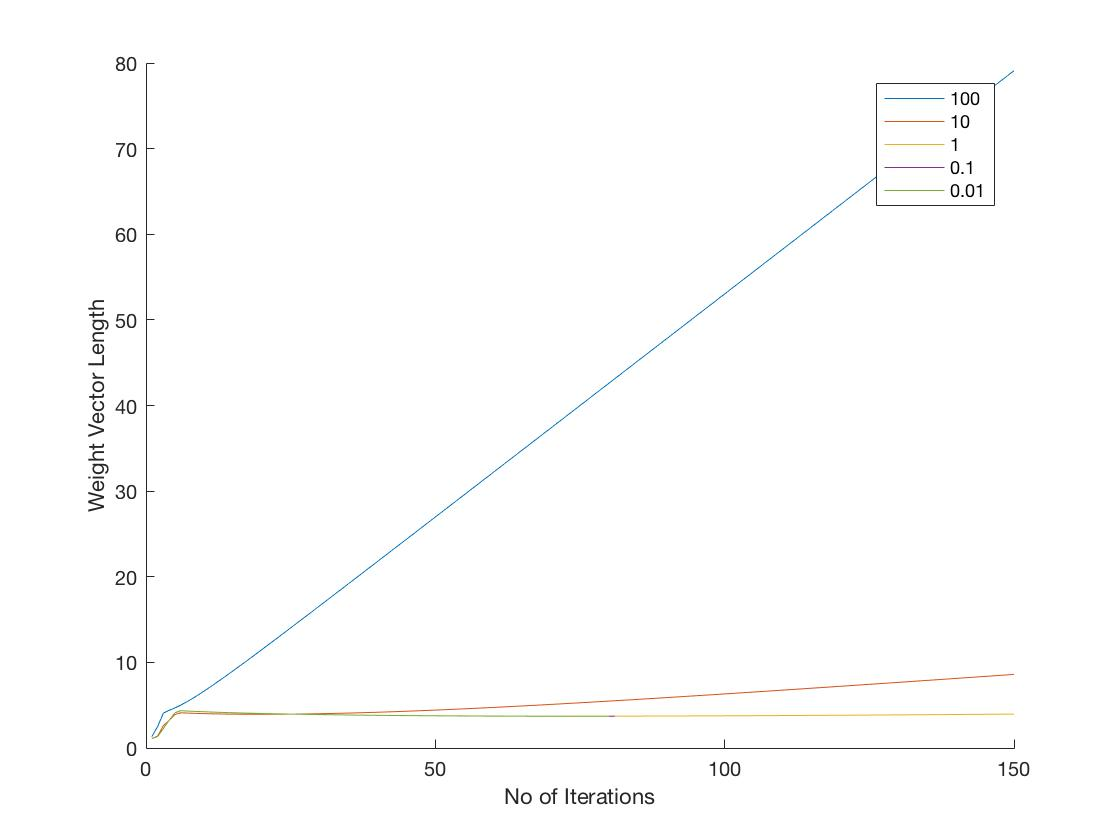
\includegraphics[width=0.45\columnwidth]{5c_l1}
  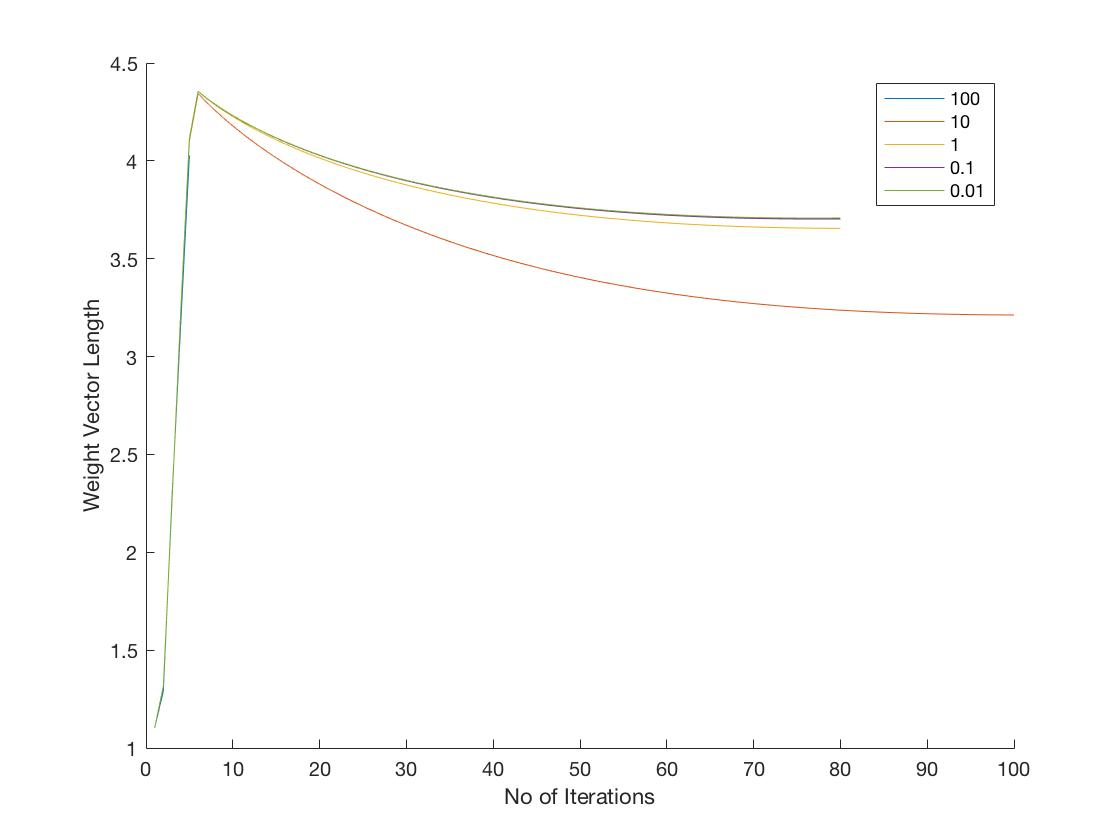
\includegraphics[width=0.45\columnwidth]{5c_l2}
  \centering
  \caption{Left: L1 Right: L2}
  \label{fig:5_c}
  \end{figure}

\item \textbf{Test set error vs. Log Lambda}\\
Test error initially increases with the log of lambda values and then starts decreasing after reaching an optimum value. This is because initially its effect is very insignificant to cause any change to the cost function. In between it reaches an optimum  and then again the regularization term starts to dominate the cost function which is highly unfavourable, so we see a steep increase in error.
\begin{figure}[H]
  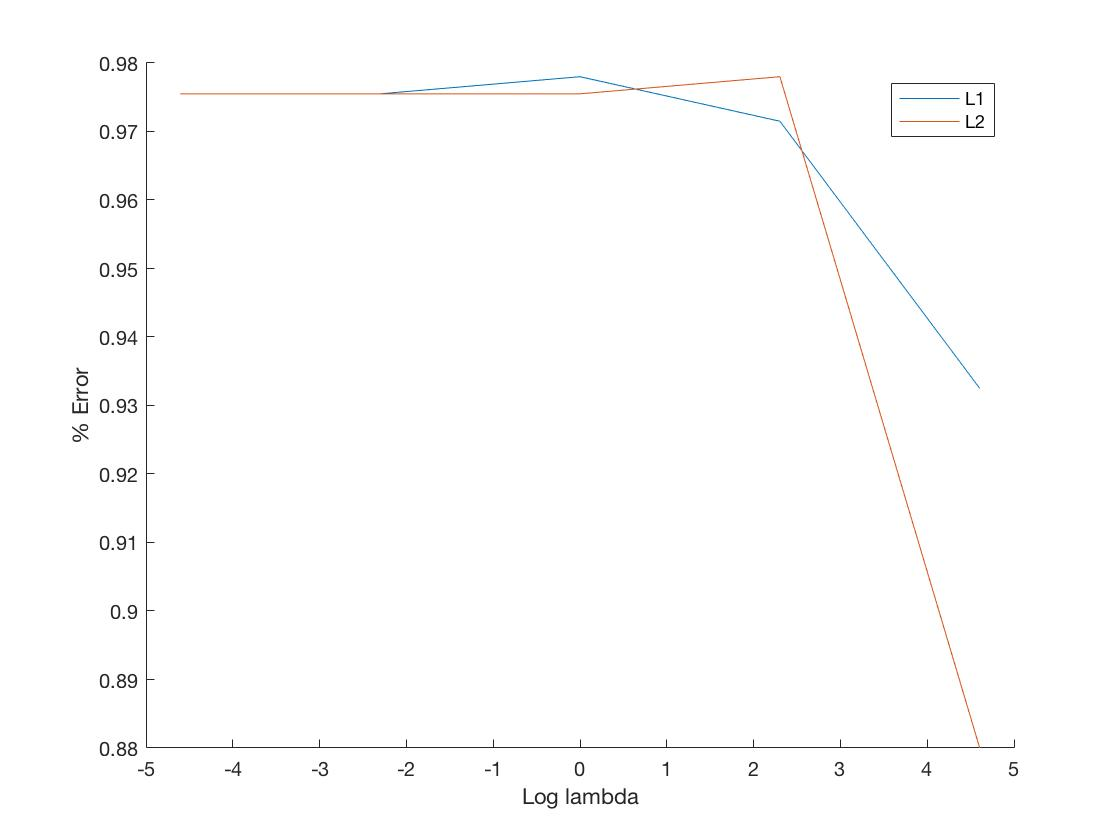
\includegraphics[width=0.6\columnwidth]{5d}
  \centering
  \caption{Error vs log lambda}
  \label{fig:5_d}
  \end{figure}

\item \textbf{L1 Regularization weight visualization}\\
We see that for large values of lambda L1 regularization shows its sparse nature. We see a sparse set of features getting  high weight values whereas most features get a weight of zero. This is typical of L1 regularization and as such it is used in feature selection and applied to places where there would be a sparse number of good features. In this classification case too it has potential to do well as only a few of the pixels among 784 are non-zero and even lesser are relevant to the classification between 2 and 3/8. We can clearly see a 2 shaped figure when lambda value is high. As lambda value goes down, the other features start getting increasing weightage.
\begin{figure}[H]
  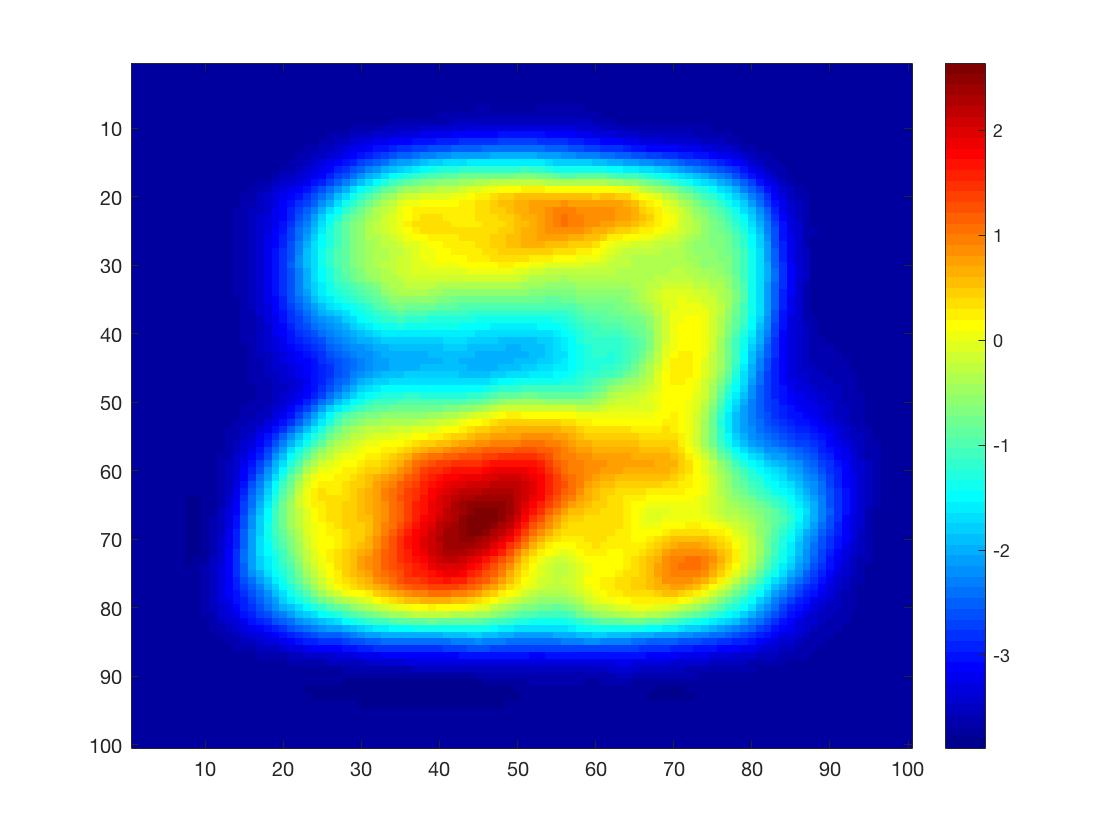
\includegraphics[width=0.45\columnwidth]{5e_1_l1}
  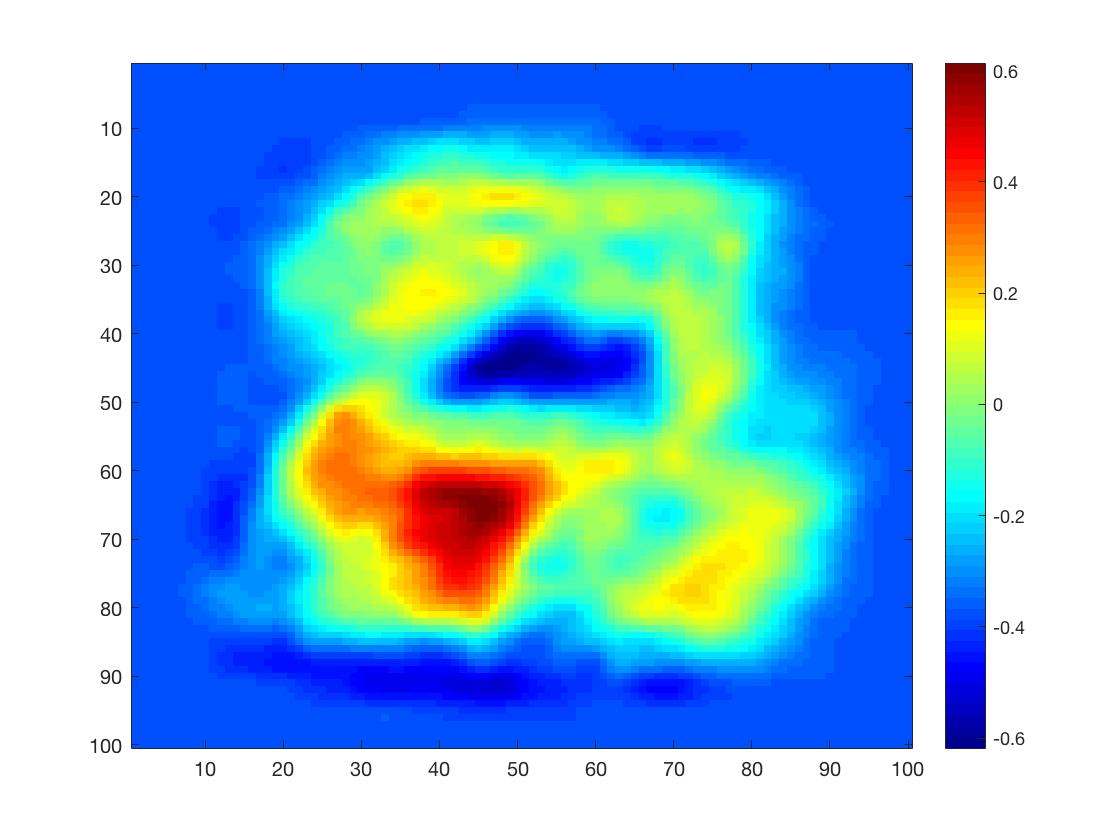
\includegraphics[width=0.45\columnwidth]{5e_2_l1}\\
  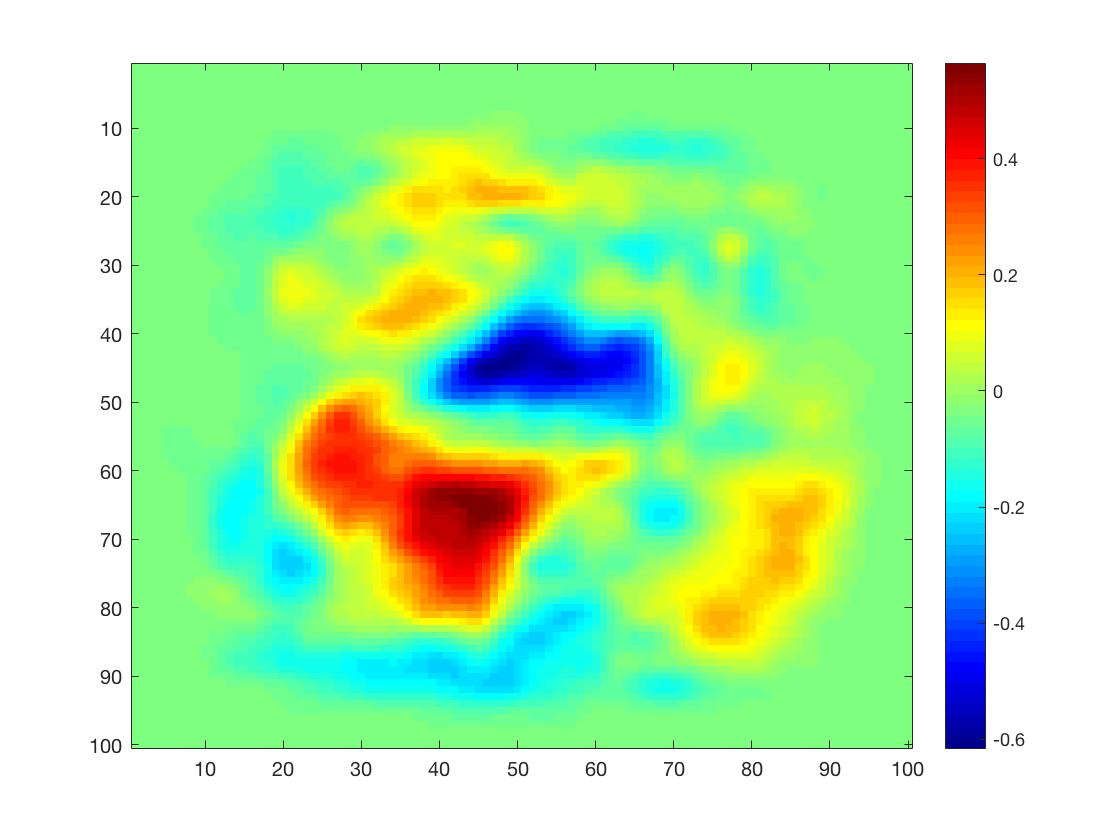
\includegraphics[width=0.45\columnwidth]{5e_3_l1}
  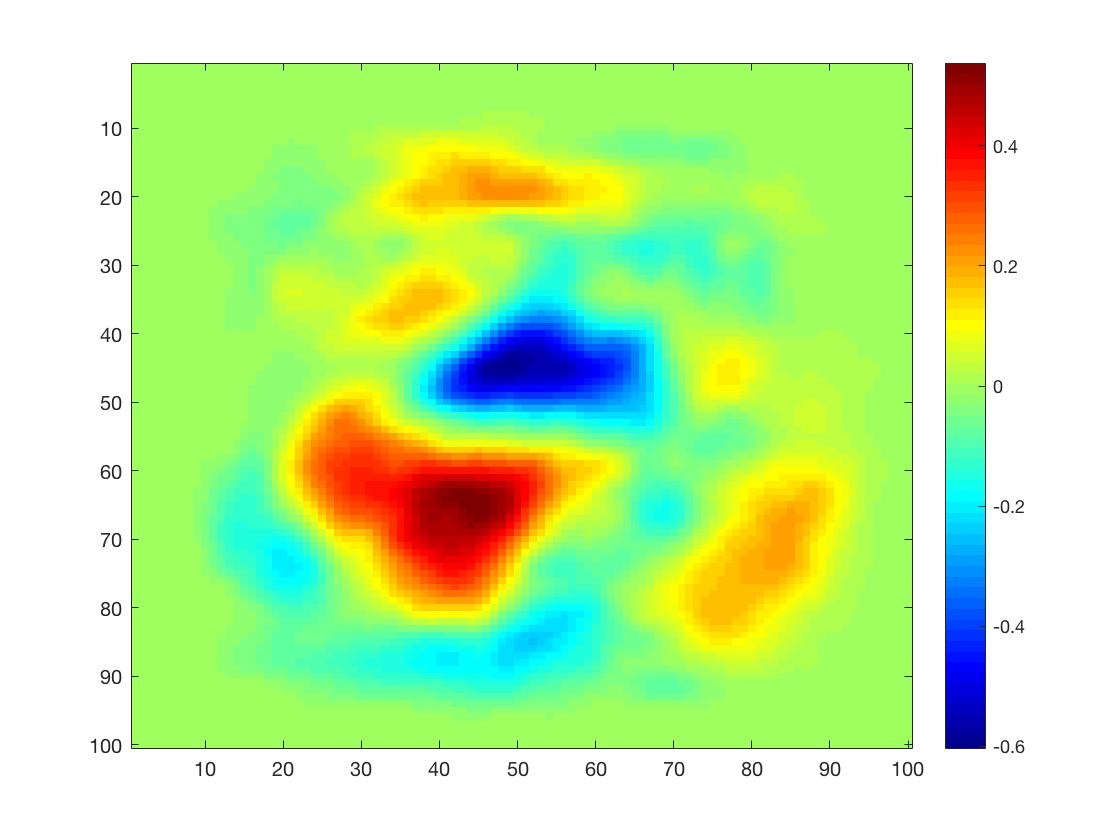
\includegraphics[width=0.45\columnwidth]{5e_4_l1}\\
  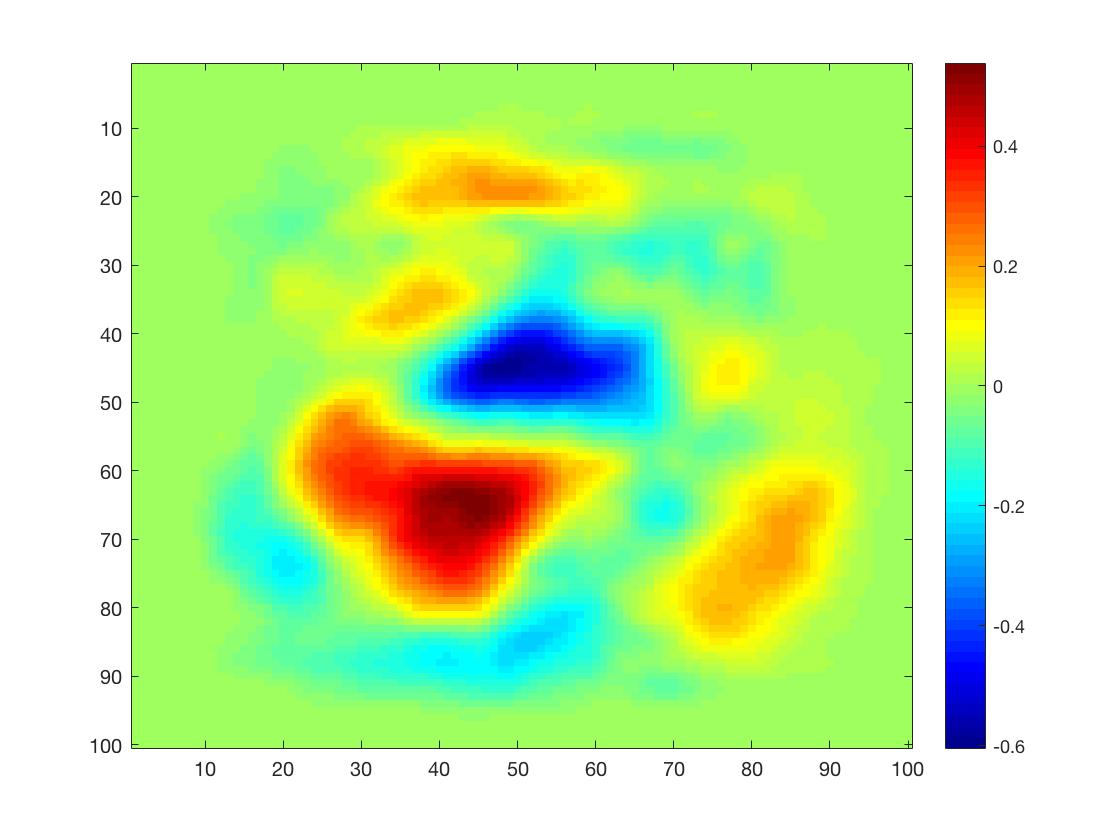
\includegraphics[width=0.45\columnwidth]{5e_5_l1}
  \centering
  \caption{L1 regularization weight visualization}
  \label{fig:5_e_l1}
  \end{figure}
  
\item \textbf{L2 Regularization weight visualization}
L2 regularization as opposed to L1 tries to favor all features evenly and as such we see that when the lambda value is high all the features have good amount of weight. The weights decrease, although slightly, as the value of lambda decreases.
\begin{figure}[H]
  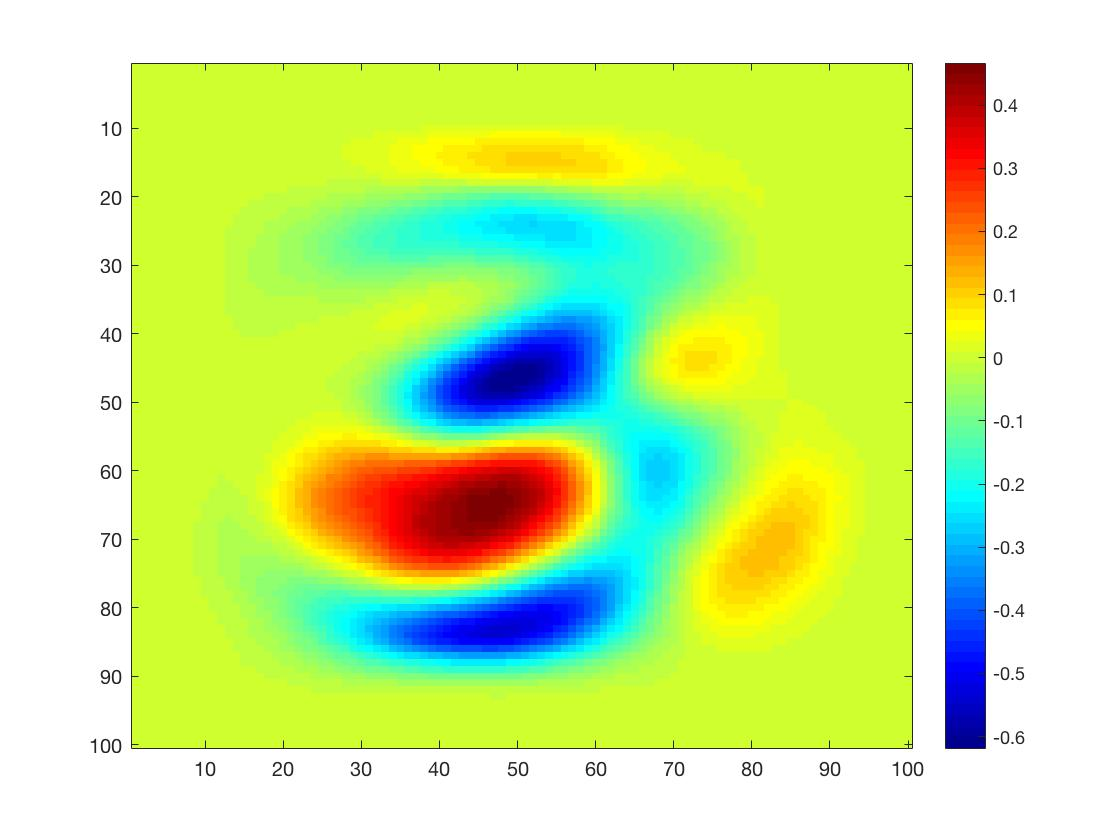
\includegraphics[width=0.45\columnwidth]{5e_1_l2}
  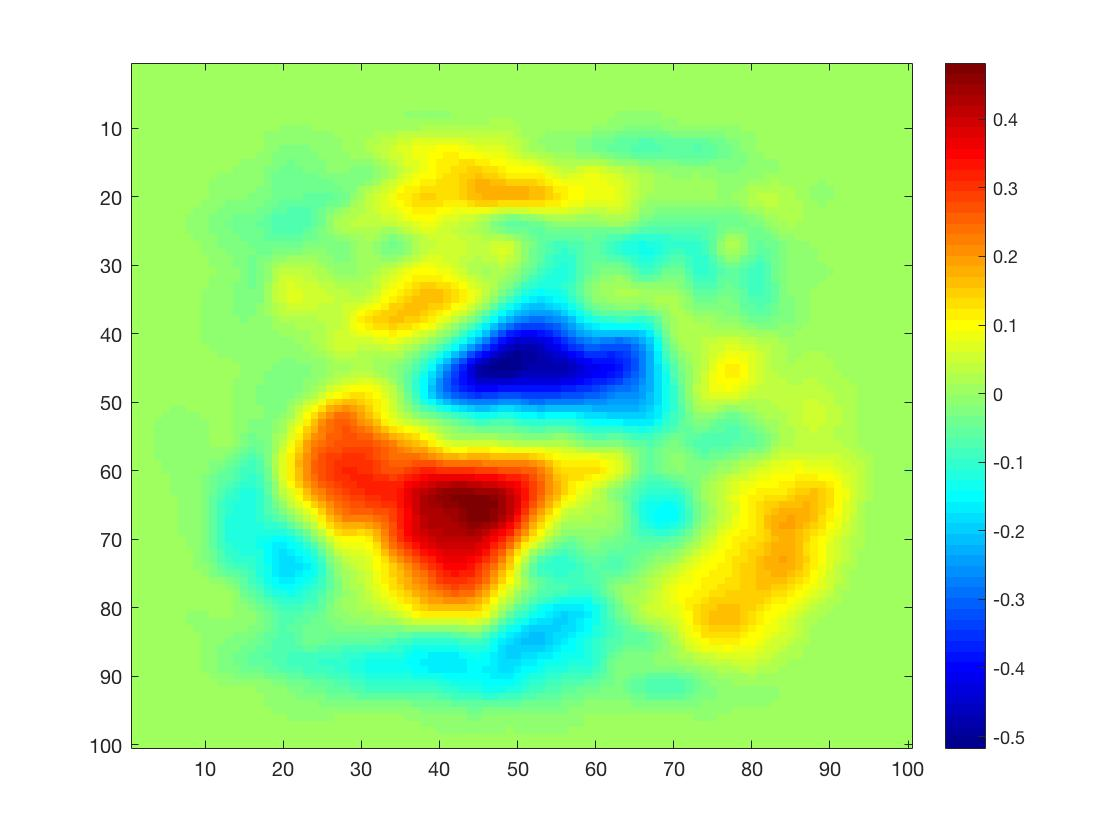
\includegraphics[width=0.45\columnwidth]{5e_2_l2}\\
  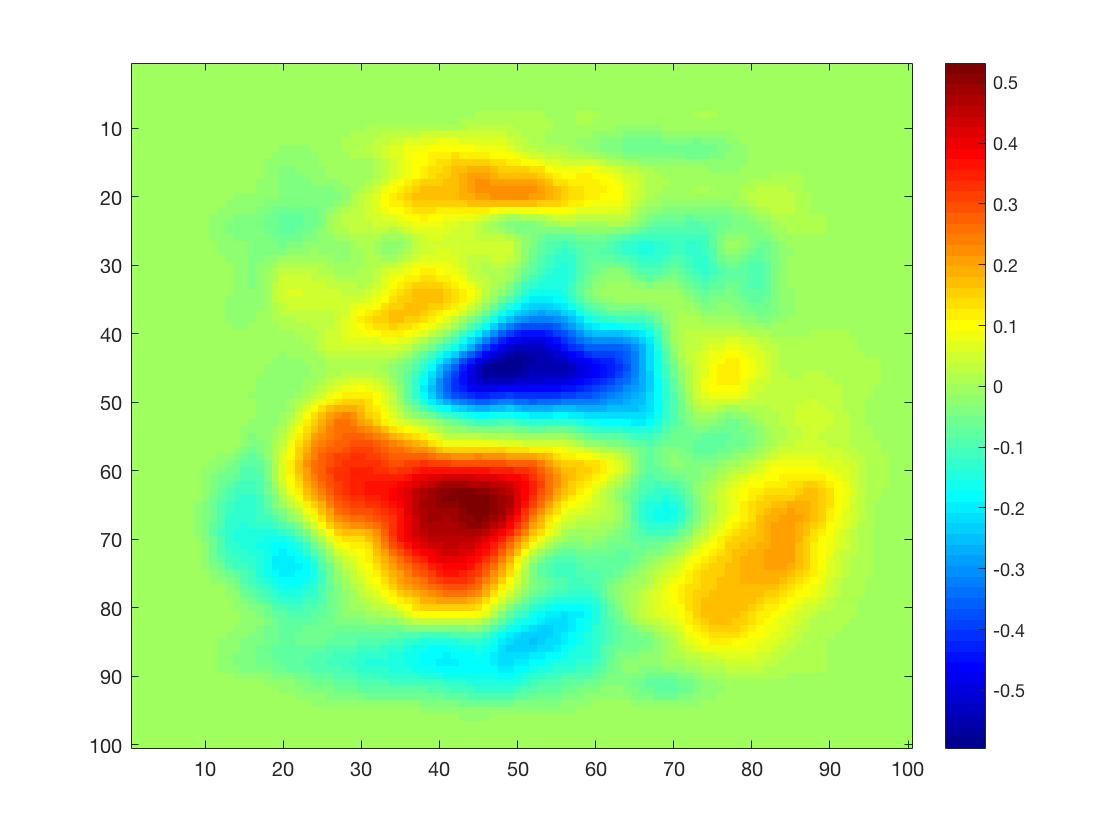
\includegraphics[width=0.45\columnwidth]{5e_3_l2}
  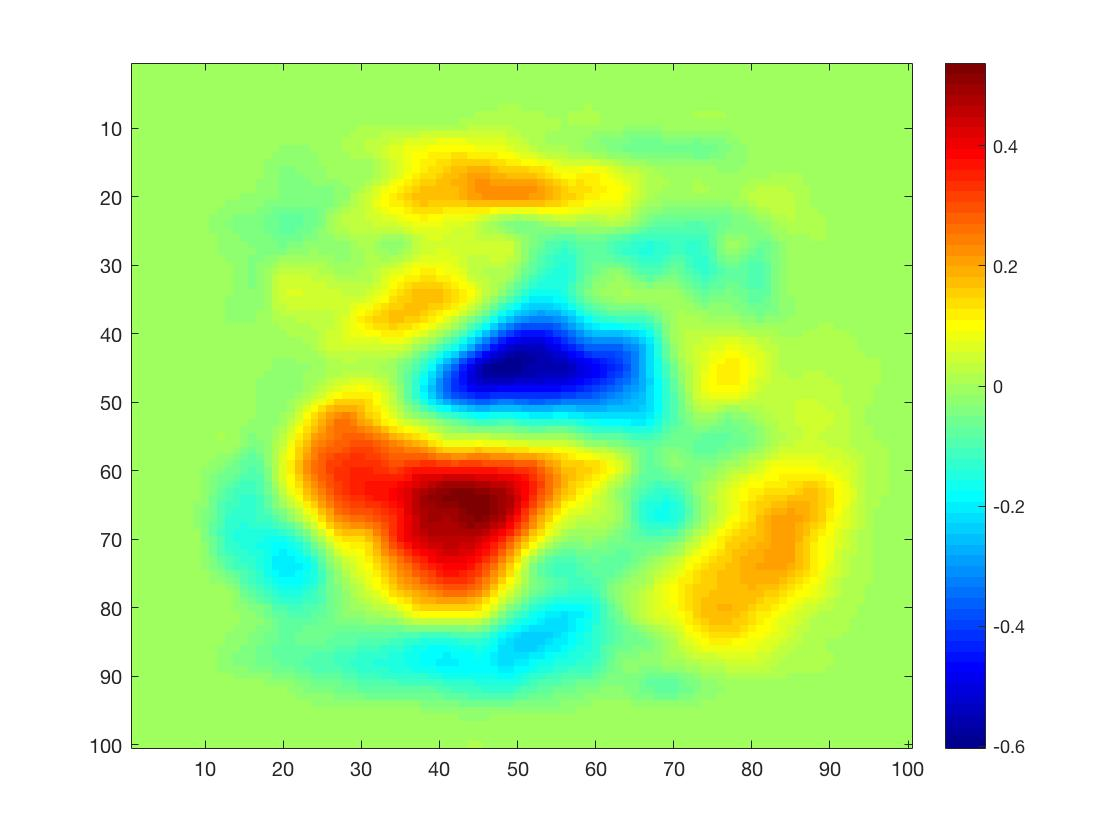
\includegraphics[width=0.45\columnwidth]{5e_4_l2}\\
  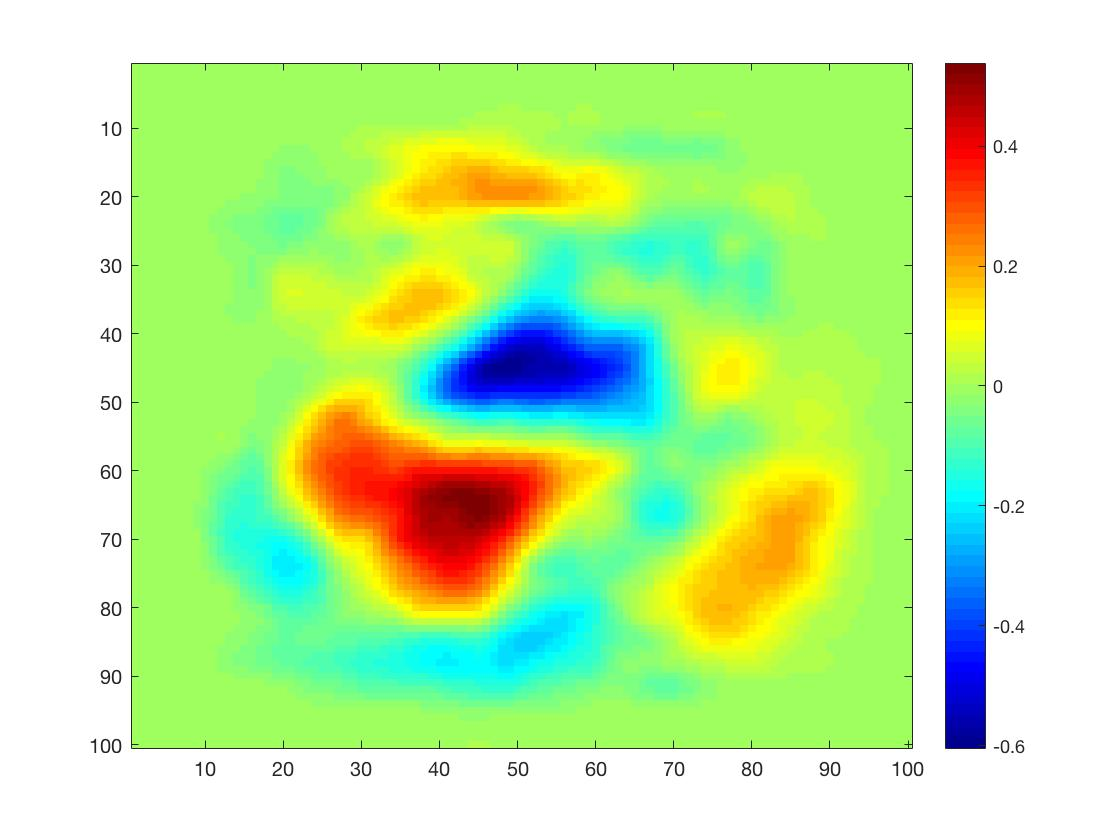
\includegraphics[width=0.45\columnwidth]{5e_5_l2}
  \centering
  \caption{L1 regularization weight visualization}
  \label{fig:5_e_l1}
  \end{figure}

\end{enumerate}
\subsection{Softmax Regression}

For all the following calculations and plots, $m = 200$, $\eta = 0.001$, $T = 2$, and $target = 2$ were used. Blue represents the training set, green the hold-out set, and red the test set. We used L1 regularization along with the $\lambda=1$, as it performed well on the test set. This could be because it is a sparse feature problem where only some pixels in the center of the image are non-zero and relevant to the classification.

The best classification accuracy achieved on the test was 86.7\%.\\

\begin{enumerate}[label=(\alph*)]

\item \textbf{Loss Function}\\
As expected the loss function, on all the three sets, gradually decreases with increasing number of iterations, in a general converging pattern.
\begin{figure}[H]
  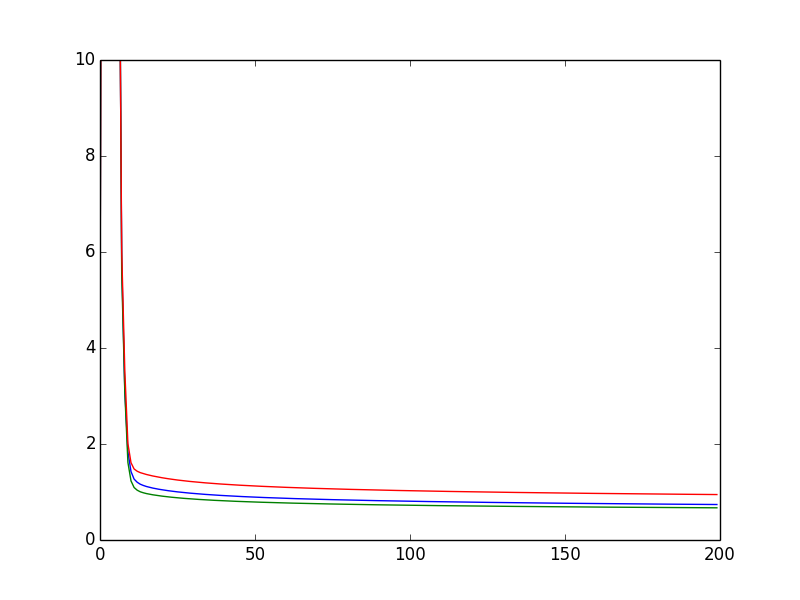
\includegraphics[width=0.45\columnwidth]{softmaxloss}
  \centering
  \caption{(Loss v/s Iterations) Loss function over the training period.}
  \label{fig:6_b}
  \end{figure}
  
\item \textbf{Percent Correct}\\  
The percentage correct classification, on all the three sets, gradually increases with increasing number of iterations, in a general converging pattern.
\begin{figure}[H]
  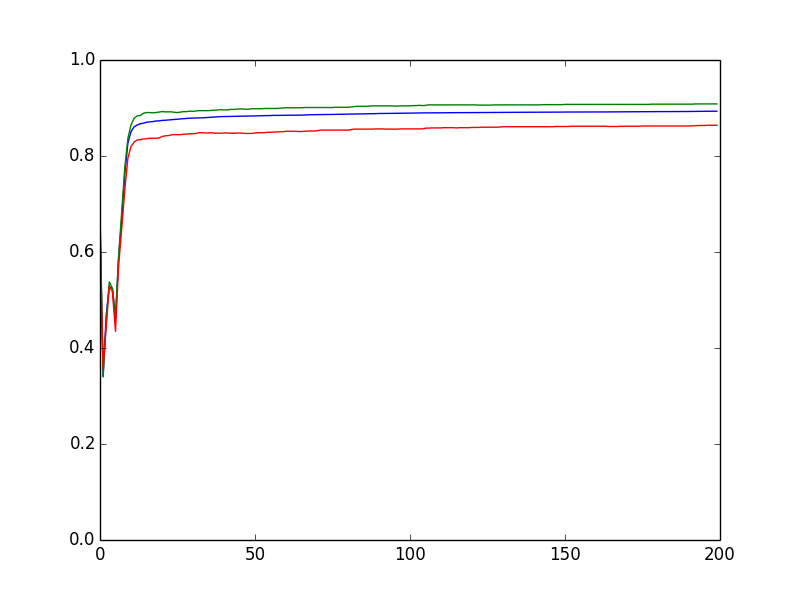
\includegraphics[width=0.45\columnwidth]{softmaxcorrect}
  \centering
  \caption{(Percent correct v/s iterations) Percent correct classifications over the training period.}
  \label{fig:6_b}
  \end{figure}
\end{enumerate}

\section{Summary}
\begin{enumerate}[label=(\alph*)]
\item We see that logistic regression is a good technique for binary classification among digits achieving accuracy of 87+\% in both 2 vs 3 and 2 vs 8.
\item Softmax regression also performs well on the multiclass classification task achieving accuracy of 87\%.
\item We see that regularization leads to better learning and thus to better classification as is demonstrated by an increase in accuracy from 96.7\% to 97.8\% on the 2 vs 3 classification task.
\item According our understanding L1 regularization is better suited for this problem as it is better at dealing with sparse features. Most elements in the feature vectors are zero in this dataset.
\item L1 regularization leads to sparser weight vectors whereas L2 regularization leads to smaller magnitude weight vectors.
\item The regularization term also has an optimum weight. As such if $\lambda$ value is too low or high, the classification error increases.
\item Looking at the results we can say that in our case the hold-out set was a pretty good representation of the test set. But we also realise that this might not always be the case as it totally depends on the dataset.

\end{enumerate}

\section{Contributions}

I, Jean Choi, did $1$ and $4$ in the homework.\\
I, Ajitesh Gupta, did $2$, $5$ and $6$ in the homework.\\

\section*{Appendix}
\lstinputlisting[language=PYTHON, caption=MATLAB source file for Problem 4 ]{cse253hw1_2vs3_jean.py}

\lstinputlisting[language=PYTHON, caption=MATLAB source file for Problem 4 ]{cse253hw1_2vs8_jean.py}

\lstinputlisting[language=MATLAB, caption=MATLAB source file for Problem 5 ]{logistic_l1.m}

\lstinputlisting[language=MATLAB, caption=MATLAB source file for Problem 5 ]{logistic_l2.m}

\lstinputlisting[language=PYTHON, caption=MATLAB source file for Problem 6 ]{softmax.py}



%\end{appendices}

\printbibliography
\end{document}
